% set the document to 12pt with A4 paper size and 1 inch margins
\documentclass[12pt,a4paper]{article}
\usepackage[utf8]{inputenc}
\usepackage{geometry}
\usepackage{hyperref}
\usepackage{graphicx}

\geometry{a4paper, margin=1in}

\title {Khidmat: TCF Alumni Pathways Project}

\author{
    Ahmed Ali \\ aa07600
    \and
    Ahsan Azeemi \\ aa07729
}
\date{12\textsuperscript{th} May 2025} 

\begin{document}
\maketitle


\section{Introduction}

\subsection{About the Khidmat}
% Use first person plural (we, us) even if you did the Khidmat individually.

% An introduction of the project, no more than 2 sentences. Provide the highest level of detail only. Other details will come later.
% Typically, "This project is to <short description of porject> for/at <client>."
This project is to develop a mobile application for The Citizens Foundation (TCF) to guide their alumni through educational and career pathways.

\subsection{About the client}
% About the client.
TCF is one of Pakistan's leading organisations in the field of education for the less privileged. TCF also maintains a dedicated alumni network and support ecosystem. \href{https://www.tcf.org.pk}{www.tcf.org.pk}.

\subsection{About the project}
% About the project.
The project involves the development of the TCF Alumni Pathways Mobile App — a user-friendly digital platform aimed at bridging the gap between TCF alumni and their academic goals. In its initial phase, the app will provide guidance on applying for matric and intermediate education, while later versions will assist alumni with university education. Deliverables include a working prototype app, a connected and populated database, an admin panel for managing the app's content and a server-side API to run the app. We will also guide on how to use and maintain the app, and provide documentation for future development.

% Syed Asfand Hussain Shah <syed.asfand@tcf.org.pk>
% Jamila Khaskheli <>
\subsection{Plan of work}
% About the plan of work.
We will follow a remote work model under the supervision of \href{mailto:jamila.khaskheli@tcf.org.pk}{Jamila Khaskheli} and \href{mailto:syed.asfand@tcf.org.pk}{Syed Asfand Hussain Shah} from TCF.With regular bi-weekly check-ins. The project will span from February to May 2025. The project will be done slowly over the course of about 8 weeks.

% Copy-paste this section with necessary modifcations for each week.
\newpage % Start the report for each week on a new page.

\section{Weekly Breakdown}

\subsection{Week 01: 27 Jan - 02 Feb 2025}
We had our first meeting with the TCF team to discuss the project. We discussed the project scope, deliverables, and timeline.

\begin{center}
    \bigskip
    \begin{tabular}{|l|l|l|l|}
        \hline
        Item 	& Activity & Time & ID \\\hline\hline
        1	& Meeting with TCF Supervisor & 1 hr(s) & aa07600, aa07729 \\\hline
    \end{tabular}

    \bigskip
    The total time spent on the Khidmat this week is as follows.

    \bigskip
    \begin{tabular}{|l|l|}
        \hline
        ID & Total Hours\\\hline\hline
        aa07600 & 1 hour(s)\\\hline
        aa07729 & 1 hour(s)\\\hline
    \end{tabular}
\end{center}

\newpage

\subsection{Week 02: 03 Feb - 09 Feb 2025}
We started working on the project. Created the SRS, reviewed the files and data shared by TCF anf finalized the proposal that was signed by TCF and submitted to the Khidmat committee.

\begin{center}
    \bigskip
    \begin{tabular}{|l|l|l|l|}
        \hline
        Item 	& Activity & Time & ID \\\hline\hline
        1	& Requirment Gathering & 2 hr(s) & aa07600, aa07729 \\\hline
        2	& Working on Proposal & 1 hr(s) & aa07600, aa07729 \\\hline
    \end{tabular}

    \bigskip
    The total time spent on the Khidmat this week is as follows.

    \bigskip
    \begin{tabular}{|l|l|}
        \hline
        ID & Total Hours\\\hline\hline
        aa07600 & 5 hour(s)\\\hline
        aa07729 & 5 hour(s)\\\hline
    \end{tabular}
\end{center}

\newpage

\subsection{Week 03: 10 Feb - 16 Feb 2025}
We created a small prototype of the app in Flutter to test the feasibility of the project.

\begin{center}
    \bigskip
    \begin{tabular}{|l|l|l|l|}
        \hline
        Item 	& Activity & Time & ID \\\hline\hline
        1	& Proof of Concept App & 3 hr(s) & aa07600, aa07729 \\\hline
    \end{tabular}

    \bigskip
    The total time spent on the Khidmat this week is as follows.

    \bigskip
    \begin{tabular}{|l|l|}
        \hline
        ID & Total Hours\\\hline\hline
        aa07600 & 3 hour(s)\\\hline
        aa07729 & 3 hour(s)\\\hline
    \end{tabular}
\end{center}

\newpage

\subsection{Week 04: 17 Feb - 23 Feb 2025}
We had a meeting with the TCF team to show them the prototype and get their feedback.

\begin{center}
    \bigskip
    \begin{tabular}{|l|l|l|l|}
        \hline
        Item 	& Activity & Time & ID \\\hline\hline
        1	& Meeting with TCF Supervisors & 1 hr(s) & aa07600, aa07729 \\\hline
    \end{tabular}

    \bigskip
    The total time spent on the Khidmat this week is as follows.

    \bigskip
    \begin{tabular}{|l|l|}
        \hline
        ID & Total Hours\\\hline\hline
        aa07600 & 1 hour(s)\\\hline
        aa07729 & 1 hour(s)\\\hline
    \end{tabular}
\end{center}

\newpage

\subsection{Week 05: 24 Feb - 02 Mar 2025}
We created the data model, figured all the features and use case scenarios and then created the database schema. We also created the API specification which will then be used to create the backend.

\begin{center}
    \bigskip
    \begin{tabular}{|l|l|l|l|}
        \hline
        Item 	& Activity & Time & ID \\\hline\hline
        1	& Data Model Creation & 2 hr(s) & aa07600, aa07729 \\\hline
        2	& Usecases and Scenario Validation & 2 hr(s) & aa07600, aa07729 \\\hline
        3	& API Specification & 3 hr(s) & aa07600, aa07729 \\\hline
    \end{tabular}

    \bigskip
    The total time spent on the Khidmat this week is as follows.

    \bigskip
    \begin{tabular}{|l|l|}
        \hline
        ID & Total Hours\\\hline\hline
        aa07600 & 7 hour(s)\\\hline
        aa07729 & 7 hour(s)\\\hline
    \end{tabular}
\end{center}

\newpage

\subsection{Week 06: 03 Mar - 09 Mar 2025}
We had a progress update meeting with the TCF team. Discussed the data model and the API specification. Made changes according to their feedback.

\begin{center}
    \bigskip
    \begin{tabular}{|l|l|l|l|}
        \hline
        Item 	& Activity & Time & ID \\\hline\hline
        1	& Meeting with TCF Supervisors & 1 hr(s) & aa07600, aa07729 \\\hline
    \end{tabular}

    \bigskip
    The total time spent on the Khidmat this week is as follows.

    \bigskip
    \begin{tabular}{|l|l|}
        \hline
        ID & Total Hours\\\hline\hline
        aa07600 & 1 hour(s)\\\hline
        aa07729 & 1 hour(s)\\\hline
    \end{tabular}
\end{center}

\newpage

\subsection{Week 07: 10 Mar - 16 Mar 2025}
Development work started. We divided the work between the backend and the app. The development of many things also required us to first learn about the technologies we are using. So it was a mix process of learning and development.

\begin{center}
    \bigskip
    \begin{tabular}{|l|l|l|l|}
        \hline
        Item 	& Activity & Time & ID \\\hline\hline
        1	& Backend - Codebase setup & 1 hr(s) & aa07600 \\\hline
        2	& Backend - User authentication APIs & 3 hr(s) & aa07600 \\\hline\hline
        3	& App - Theme and structure research & 2 hr(s) & aa07729 \\\hline
        4	& App - Mvvm architecture setup & 1 hr(s) & aa07729 \\\hline
        5	& App - Color theme and dark/light theme setup & 2 hr(s) & aa07729 \\\hline
    \end{tabular}

    \bigskip
    The total time spent on the Khidmat this week is as follows.

    \bigskip
    \begin{tabular}{|l|l|}
        \hline
        ID & Total Hours\\\hline\hline
        aa07600 & 4 hour(s)\\\hline
        aa07729 & 5 hour(s)\\\hline
    \end{tabular}
\end{center}

\newpage

\subsection{Week 08: 17 Mar - 23 Mar 2025}
Development work continued. We created the database and the schema. We also created the user management APIs. The app was also started and we created the home page and the settings page.

\begin{center}
    \bigskip
    \begin{tabular}{|l|l|l|l|}
        \hline
        Item 	& Activity & Time & ID \\\hline\hline
        1	& MongoDB Database created with schema & 2 hr(s) & aa07600 \\\hline
        2	& Data given by TCT cleaned and analysed & 1 hr(s) & aa07600 \\\hline
        3	& Backend - User management APIs & 3 hr(s) & aa07600 \\\hline\hline
        4	& App - Home page & 3 hr(s) & aa07729 \\\hline
        5	& App - Notifications (static) & 2 hr(s) & aa07729 \\\hline
        6	& App - Settings screen & 1 hr(s) & aa07729 \\\hline
        7	& App - Device UUID registration & 1 hr(s) & aa07729 \\\hline
    \end{tabular}

    \bigskip
    The total time spent on the Khidmat this week is as follows.

    \bigskip
    \begin{tabular}{|l|l|}
        \hline
        ID & Total Hours\\\hline\hline
        aa07600 & 6 hour(s)\\\hline
        aa07729 & 7 hour(s)\\\hline
    \end{tabular}
\end{center}

\newpage

\subsection{Week 09: 24 Mar - 30 Mar 2025}
No work was done this week due to last week of Ramadan and course workloads.

\begin{center}
    \bigskip
    \begin{tabular}{|l|l|l|l|}
        \hline
        Item 	& Activity & Time & ID \\\hline\hline
        - & - & - & - \\\hline
    \end{tabular}

    \bigskip
    The total time spent on the Khidmat this week is as follows.

    \bigskip
    \begin{tabular}{|l|l|}
        \hline
        ID & Total Hours\\\hline\hline
        aa07600 & -\\\hline
        aa07729 & -\\\hline
    \end{tabular}
\end{center}

\newpage

\subsection{Week 10: 31 Mar - 06 Apr 2025}
No work was done this week due to Eid holidays.

\begin{center}
    \bigskip
    \begin{tabular}{|l|l|l|l|}
        \hline
        Item 	& Activity & Time & ID \\\hline\hline
        - & - & - & - \\\hline
    \end{tabular}

    \bigskip
    The total time spent on the Khidmat this week is as follows.

    \bigskip
    \begin{tabular}{|l|l|}
        \hline
        ID & Total Hours\\\hline\hline
        aa07600 & -\\\hline
        aa07729 & -\\\hline
    \end{tabular}
\end{center}

\newpage

\subsection{Week 11: 07 Apr - 13 Apr 2025}
We had a progress update meeting with the TCF team. We demoed the app and shared the current working version of the app. We also discussed the next steps and the timeline for the project.

\begin{center}
    \bigskip
    \begin{tabular}{|l|l|l|l|}
        \hline
        Item 	& Activity & Time & ID \\\hline\hline
        1	& Meeting with TCF Supervisor  & 1 hr(s) & aa07600, aa07729 \\\hline
    \end{tabular}

    \bigskip
    The total time spent on the Khidmat this week is as follows.

    \bigskip
    \begin{tabular}{|l|l|}
        \hline
        ID & Total Hours\\\hline\hline
        aa07600 & 1 hour(s)\\\hline
        aa07729 & 1 hour(s)\\\hline
    \end{tabular}
\end{center}

\newpage

\subsection{Week 12: 14 Apr - 20 Apr 2025}
Main development focus on institute features on both the backend and the app. The admin panel dashboard was intialized.

\begin{center}
    \bigskip
    \begin{tabular}{|l|l|l|l|}
        \hline
        Item 	& Activity & Time & ID \\\hline\hline
        1	& Backend - Institute management APIs & 5 hr(s) & aa07600 \\\hline
        2	& Backend - Institute Rating APIs & 2 hr(s) & aa07600 \\\hline
        3	& Admin panel - Codebase setup & 1 hr(s) & aa07600 \\\hline
        4	& Admin panel - Main dashboard & 3 hr(s) & aa07600 \\\hline\hline
        5	& App - Student search settings form & 3 hr(s) & aa07729 \\\hline
        6	& App - Mapbox api documentation and research for pricing model & 1 hr(s) & aa07729 \\\hline
        7	& App - find institutes screen & 2 hr(s) & aa07729 \\\hline
        8	& App - Institute view on map via mapbox api screen & 5 hr(s) & aa07729 \\\hline
        9	& App - Iinstitue favorites screen & 2 hr(s) & aa07729 \\\hline
    \end{tabular}

    \bigskip
    The total time spent on the Khidmat this week is as follows.

    \bigskip
    \begin{tabular}{|l|l|}
        \hline
        ID & Total Hours\\\hline\hline
        aa07600 & 11 hour(s)\\\hline
        aa07729 & 13 hour(s)\\\hline
    \end{tabular}
\end{center}

\newpage

\subsection{Week 13: 21 Apr - 27 Apr 2025}
No work was done this week due to final week of classes and course workloads.

\begin{center}
    \bigskip
    \begin{tabular}{|l|l|l|l|}
        \hline
        Item 	& Activity & Time & ID \\\hline\hline
        - & - & - & - \\\hline
    \end{tabular}

    \bigskip
    The total time spent on the Khidmat this week is as follows.

    \bigskip
    \begin{tabular}{|l|l|}
        \hline
        ID & Total Hours\\\hline\hline
        aa07600 & -\\\hline
        aa07729 & -\\\hline
    \end{tabular}
\end{center}

\newpage

\subsection{Week 14: 28 Apr - 04 May 2025}
We had a progress update meeting with the TCF team.

\begin{center}
    \bigskip
    \begin{tabular}{|l|l|l|l|}
        \hline
        Item 	& Activity & Time & ID \\\hline\hline
        1	& Meeting with TCF Supervisor  & 1 hr(s) & aa07600, aa07729 \\\hline
    \end{tabular}

    \bigskip
    The total time spent on the Khidmat this week is as follows.

    \bigskip
    \begin{tabular}{|l|l|}
        \hline
        ID & Total Hours\\\hline\hline
        aa07600 & 1 hour(s)\\\hline
        aa07729 & 1 hour(s)\\\hline
    \end{tabular}
\end{center}

\newpage

\subsection{Week 15: 05 May - 11 May 2025}
Many other core features were worked on. Development of backend almost completed and admin panel was updated. The app was also updated with the new features. The deployment of the backend and admin panel was also done on Digital Ocean.

\begin{center}
    \bigskip
    \begin{tabular}{|l|l|l|l|}
        \hline
        Item 	& Activity & Time & ID \\\hline\hline
        1	& Backend - AppFeedback APIs & 2 hr(s) & aa07600 \\\hline
        2	& Backend - Institute Add requests APIs & 1 hr(s) & aa07600 \\\hline
        3	& Backend - Admin dashboard APIs & 3 hr(s) & aa07600 \\\hline
        4	& Backend - Resource management APIs & 2 hr(s) & aa07600 \\\hline
        5	& Admin panel - User management & 2 hr(s) & aa07600 \\\hline
        6	& Admin panel - Institute management & 3 hr(s) & aa07600 \\\hline\hline
        7	& App - Saving favorites insitute & 2 hr(s) & aa07729 \\\hline
        8	& App - Institute add request form & 2 hr(s) & aa07729 \\\hline
        9	& App - Institute details screen & 2 hr(s) & aa07729 \\\hline
        10  & App - Release size optimization, branding updated & 2 hr(s) & aa07729 \\\hline
        11  & App - Backward compatibility check & 2 hr(s) & aa07729 \\\hline\hline
        12  & Backend and Admin Panel deployed on Cloud & 3 hr(s) & aa07600, aa07729 \\\hline
    \end{tabular}

    \bigskip
    The total time spent on the Khidmat this week is as follows.

    \bigskip
    \begin{tabular}{|l|l|}
        \hline
        ID & Total Hours\\\hline\hline
        aa07600 & 16 hour(s)\\\hline
        aa07729 & 13 hour(s)\\\hline
    \end{tabular}
\end{center}

\newpage

\subsection{Week 16: 12 May - 18 May 2025}
We had a demo meeting with the TCF team. Shared the admin panel and app package with them. We now completed all the other remaining features of the app.

\begin{center}
    \bigskip
    \begin{tabular}{|l|l|l|l|}
        \hline
        Item 	& Activity & Time & ID \\\hline\hline
        1	& Meeting with TCF Supervisors  & 1 hr(s) & aa07600, aa07729 \\\hline\hline
        2	& Backend - Notification APIs + Firebase integration & 2 hr(s) & aa07600 \\\hline
        3	& Admin panel - Institute rating management & 1 hr(s) & aa07600 \\\hline
        4	& Admin panel - Resource management & 1 hr(s) & aa07600 \\\hline
        5	& Admin panel - App feedback management & 1 hr(s) & aa07600 \\\hline
        6	& Admin panel - Institute add requests management & 1 hr(s) & aa07600 \\\hline\hline
        7	& App - Institute rating screen & 1 hr(s) & aa07729 \\\hline
        8	& App - Resource screen dynamically updated & 1 hr(s) & aa07729 \\\hline
        9	& App - Live push notifications & 2 hr(s) & aa07729 \\\hline
    \end{tabular}

    \bigskip
    The total time spent on the Khidmat this week is as follows.

    \bigskip
    \begin{tabular}{|l|l|}
        \hline
        ID & Total Hours\\\hline\hline
        aa07600 & 7 hour(s)\\\hline
        aa07729 & 5 hour(s)\\\hline
    \end{tabular}
\end{center}

\newpage

\section{Conclusion}

% Remind the reader about the project. Summarise your activities over the course of the project.
The project was to develop a mobile application for The Citizens Foundation (TCF) to guide their alumni through educational and career pathways. The project was to create a MVP of the alumni pathways app system to propose the project to higher management. We will continue on the project on testing, bug fixing and maintenance. Over the course of the project we learned about a lot of different technologies and tools. We also learned about the importance of documentation and how to work in a team. We also learned about the importance of communication and how to work with a client. The project was a great learning experience for us and we are grateful to TCF for giving us this opportunity. Special thanks to our supervisors, namely Jamila Khaskheli and Syed Asfand Hussain Shah, for their guidance and support throughout the project.

\newpage
\thispagestyle{empty}
% Show your external supervisor your report, especially the weekly upates; have them sign a printed copy of this page; scan the signed page; and include the scanned page in this document as an image.

\begin{center}
  {\Large\bf Khidmat Completion Form}\\[5pt]
  \small To be completed by the external supervisor.  
\end{center}
\bigskip

\noindent{\it Please use the space below to provide any comments you may have on the students' performance, the Khidmat program, or any other feedback you want to share with Habib University's Khidmat committee. We can also be reached at \href{mailto:khidmat@sse.habib.edu.pk}{khidmat@sse.habib.edu.pk}.}

\begin{figure}[h]
    \centering
    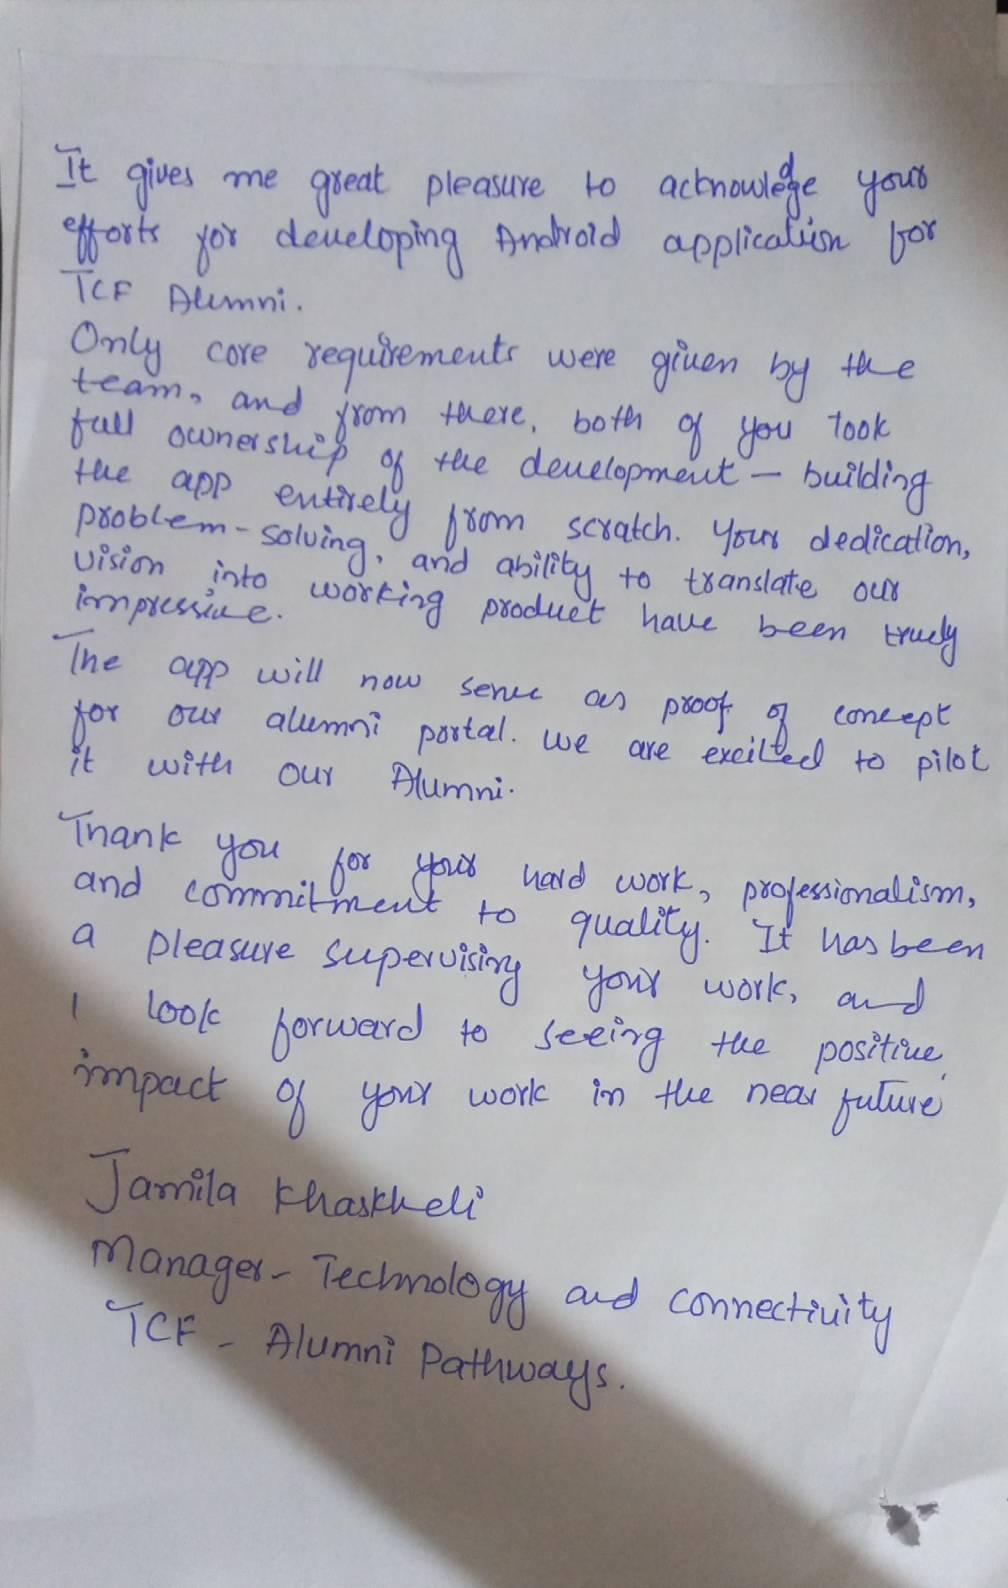
\includegraphics[width=0.6\textwidth]{comments.jpg}
\end{figure}

I hereby certify that I supervised Ahmed Ali and Ahsan Azeemi for the Khidmat described in this report. Furthermore, that I have read and agree with the weekly updates included in this report. My signature below marks the successful completion of the work undertaken for the Khidmat.\\
\bigskip
\bigskip

\noindent\begin{tabular}{@{}p{.6\textwidth}@{\hspace{.1\textwidth}}p{.3\textwidth}}
  \hrulefill &   \hrulefill \\
  Name and signature & Location and date
\end{tabular}

\end{document}
